\documentclass{beamer}
\usetheme{Boadilla}
\usecolortheme{whale}
\usepackage{tikz,pgfplots,graphicx}
\usepackage{amsmath,amssymb,amsthm,amsfonts,mathtools}
\usepackage{algorithm,algorithmicx,algpseudocode}
\usepackage{adjustbox}
\usepackage{subcaption}
\usepackage{multirow,pbox}
\usefonttheme[onlymath]{serif}
\usepackage[retainorgcmds]{IEEEtrantools}
\usetikzlibrary{shapes.geometric, arrows}


\tikzstyle{startstop} = [rectangle, rounded corners, minimum width=0.5cm, minimum height=0.5cm,text centered, draw=black]
\tikzstyle{process} = [rectangle, minimum width=0.5cm, minimum height=0.5cm, text centered, draw=black]
\tikzstyle{decision} = [diamond, minimum width=0.5cm, minimum height=0.5cm, text centered, draw=black]
\tikzstyle{arrow} = [thick,->,>=stealth]
\tikzstyle{cy}=[cylinder, alias=cyl, aspect=0.2, shape border rotate=90, minimum width=2cm, minimum height=1cm, text centered, draw=black]
\tikzstyle{rec}=[rectangle, rounded corners=0.25cm, minimum width=2cm, minimum height=0.3cm, text centered, draw=black]
\tikzstyle{arrow}=[thick,->,>=stealth]
\tikzstyle{E} = [draw=black,minimum width=1cm,minimum height=1cm,node distance=1cm]
\pgfdeclarelayer{background}
\pgfdeclarelayer{foreground}
\pgfsetlayers{background,main,foreground}



\title[A GA Based MKL Algorithm]{A Genetic Algorithm Based\\ Multiple Kernel Learning Algorithm}
      \author[Wang Fan]{Wang Fan\\
      \vspace{0.5cm}Supervisor: Assoc.~Prof.~Chua Chek Beng\vspace{1cm}}
\institute[NTU]{Division of Mathematical Sciences\\
        School of Physical and Mathematical Sciences\\
        Nanyang Technological University\\
        Singapore}
\date{20 April 2016}

\begin{document}
	\frame{\titlepage}
	
	\begin{frame}
		\frametitle{Introduction}
		\only<1>{
			\begin{figure}
				\includegraphics[width=0.8\textwidth]{Pictures/face}
			\end{figure}}
		\only<2>{
			\begin{figure}
				\includegraphics[width=0.8\textwidth]{Pictures/facedetection}
			\end{figure}}
		\only<3>{
			\begin{figure}
				\includegraphics[width=0.8\textwidth]{Pictures/classification}
			\end{figure}
			}
	\end{frame}
	
	\begin{frame}
		\frametitle{Outline}
		\tableofcontents
	\end{frame}
	
	\AtBeginSection[]
	{
		\begin{frame}
	    	\frametitle{Outline}
			\tableofcontents[currentsection]
		\end{frame}
	}
	
	
	\section{Introduction}
	\begin{frame}
		\frametitle{Motivation}
		\centering
		\only<1>{
			\includegraphics[width=0.5\textwidth]{Pictures/linearclass}
			}
		\only<2>{
			\includegraphics[width=0.5\textwidth]{Pictures/nonlinearclass}
			}
				
	\end{frame}
	
	\begin{frame}
		\frametitle{Motivation}
		\begin{itemize}	
			\item<1-> Kernel method
			\begin{itemize}
				\item mapping data to a \alert{feature space}$\quad\Longrightarrow \quad$data are linear separable\par
				
				\only<1>{
					\begin{block}{Kernel}
						A kernel is a function $K$ that for all $\mathbf{x},\mathbf{x}'\in\mathbb{R}^n$ satisfies
						\begin{equation*}
							K(\mathbf{x},\mathbf{x}')=\Phi(\mathbf{x})\cdot\Phi(\mathbf{x}'),
						\end{equation*}
						where $\Phi$ is a mapping from $\mathbb{R}^n$ to Hilbert space $\mathcal{H}$, i.e. $\displaystyle\Phi:\mathbf{x} \mapsto\Phi(\mathbf{x})\in \mathcal{H}$.
					\end{block}
					\begin{minipage}{0.35\textwidth}
						\includegraphics[width=0.8\textwidth]{Pictures/nonlinearclass}
					\end{minipage}
					$\Rightarrow$
					\begin{minipage}{0.35\textwidth}
						\includegraphics[width=0.8\textwidth]{Pictures/linearclass}
					\end{minipage}
					}
			\end{itemize}
			\only<2>{
				\item Support Vector Machine looks for a hyperplane that maximizes the distance between two classes.\par
				\vspace{1cm}
				\centering
				\includegraphics[width=0.4\textwidth]{Pictures/svm}
				}
			\only<3>{
				\item Support Vector Machine
				\begin{itemize}
					\item Standard SVM:
					\begin{IEEEeqnarray}{ll}{\label{eqn:svmprimal}}
						\min_{\mathbf{w},\xi,b}\qquad&\frac{1}{2}\|\mathbf{w}\|^2+C\sum_{i=1}^n\xi_i\nonumber\\
						\text{s.t.} &y_i((\mathbf{w}\cdot \Phi(x_i))-b)\geq1-\xi_i,  i=1,2,\ldots ,n\nonumber\\
						&\xi_i\geq0,  i=1,2,\ldots,n,\nonumber
					\end{IEEEeqnarray}
					\item Dual form:
					\begin{IEEEeqnarray}{ll} \label{eqn:svmdual}
						\max_{\alpha}\qquad & -\frac{1}{2}\sum_{i=1}^n\sum_{j=1}^n y_i y_j\Big(\Phi(x_i)\cdot \Phi(x_j)\Big)\alpha_i\alpha_j+\sum_{j=1}^n \alpha_j\nonumber\\
						\text{s.t.}\qquad &\sum_{i=1}^n \alpha_i y_i=0,\nonumber\\ 
						&0\leq\alpha_i\leq C,~i=1,\ldots,n	 \nonumber
					\end{IEEEeqnarray}
				\end{itemize}
			}
			\item<4-> Problem of kernel methods, in particular, SVM:
		    \begin{itemize}
				\item How to choose a `good' kernel?
			\end{itemize}
			\item<5-> Multiple kernel learning is one solution.
		\end{itemize}
	\end{frame}
	
	\begin{frame}[label=primal]
		\frametitle{Motivation}
		\begin{itemize}
			\item<1-> Multiple kernel learning
			\begin{itemize}
				\item MKL learns a linear combination of predefined kernels
				\only<1>{
					\begin{equation*}
						K(\mathbf{x},\mathbf{x}')=\sum_{k=1}^M \mu_k K_k(\mathbf{x},\mathbf{x}')
					\end{equation*}
					}
				\only<2>{
					\item Primal form: 
					\hyperlink{sec3<1>}{\beamerreturnbutton{Go Back}}
					\begin{IEEEeqnarray}{ll}
						\min_{\mathbf{w},b,\xi,\boldsymbol{\mu}}\qquad &\frac{1}{2}\sum_{k=1}^M \frac{\|\mathbf{w}_k\|^2}{\mu_k}+C\sum_{i=1}^n \xi_i\nonumber\\
						\text{s.t.} &y_i(\sum_{k=1}^M (\mathbf{w}_k\cdot\Phi_k(x_i))+b)\geq1-\xi_i,~\forall i=1,\ldots,n\nonumber \\
						&\xi_i\geq0,~\forall i=1,\ldots,n \nonumber\\
						&\sum_{k=1}^M \mu_k =1,~\mu_k\geq0,~\forall k=1,\ldots,M.\nonumber
					\end{IEEEeqnarray}	
					}
				\only<3>{
					\item Dual form:
			\begin{IEEEeqnarray}{ll}\label{eqn:mkldual}
				\max_{\alpha,\lambda}\qquad &\sum_{i=1}^n \alpha_i -\lambda\nonumber\\
				\text{s.t.}&\frac{1}{2}\sum_{i=1}^n\sum_{j=1}^n \alpha_i\alpha_j y_i y_j K_k(x_i,x_j)\leq\lambda,~\forall k=1,\ldots,M.\nonumber\\
				&\sum_{i=1}^n \alpha_i y_i=0, \nonumber\\
				&0\leq\alpha_i\leq C,~\forall i=1,\ldots,n, \nonumber
			\end{IEEEeqnarray}
			\item Quadratically Constrained Linear Programming
			}
			\end{itemize} 
			\item<4-> Problems of multiple kernel learning:
			\begin{itemize}
				\item What predefined kernels to choose?
				\item Can we tune kernel parameters automatically?
			\end{itemize}
			\item<5-> Genetic Algorithm
		\end{itemize}
	\end{frame}
		
	\begin{frame}
		\frametitle{Genetic Algorithm}
		\begin{itemize}
			\item Inspired by Darwin's theory about evolution
			\pause
			\begin{figure}
				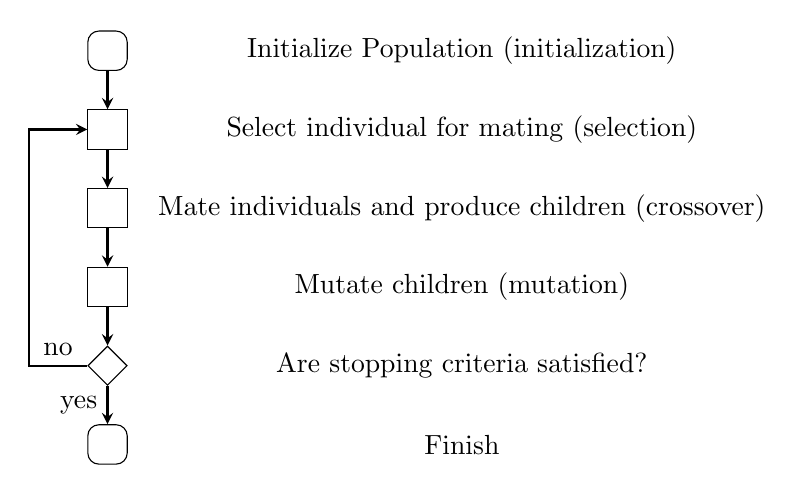
\begin{tikzpicture}[node distance=1cm]
					\node (start) [startstop] {};
					\node (p1) [process, below of=start] {};
					\node (p2) [process, below of=p1] {};
					\node (p3) [process, below of=p2] {};
					\node (dec) [decision, below of=p3] {};
					\node (end) [startstop, below of=dec] {};
					\node (l2) [coordinate, left of=dec] {};
					\node (l1) [coordinate, left of=p1] {};
					\node (d1) [right of=start, xshift=3.5cm, align=left] {Initialize Population (initialization)};
					\node (d2) [right of=p1, xshift=3.5cm] {Select individual for mating (selection)};
					\node (d3) [right of=p2, xshift=3.5cm] {Mate individuals and produce children (crossover)};
					\node (d4) [right of=p3, xshift=3.5cm] {Mutate children (mutation)};
					\node (d5) [right of=dec, xshift=3.5cm] {Are stopping criteria satisfied?};
					\node (d6) [right of=end, xshift=3.5cm] {Finish};
					\draw [arrow] (start)--(p1);
					\draw [arrow] (p1)--(p2);
					\draw [arrow] (p2)--(p3);
					\draw [arrow] (p3)--(dec);
					\draw [arrow] (dec)--node[anchor=east] {yes} (end);
					\path[draw,arrow] (dec)--node[anchor=south] {no}(l2)--(l1)--(p1);
				\end{tikzpicture}
			\end{figure}
		\end{itemize}
	\end{frame}
	
	\section{GA Based MKL Algorithm}
	\begin{frame}
		\frametitle{Overview}
		\begin{minipage}{0.48\textwidth}
			\begin{figure}
				\includegraphics[width=\textwidth]{Pictures/gamkl.png}
			\end{figure}
		\end{minipage}
		\pause
		\begin{minipage}{0.48\textwidth}
			\begin{itemize}
				\item Problems remaining
				\begin{itemize}
					\item Determine fitness function
					\item Encode parameters
					\item Solve MKL problems
				\end{itemize}
			\end{itemize}
		\end{minipage}
	\end{frame}
	
	\begin{frame}
		\frametitle{Methodology}
		\begin{minipage}{0.45\textwidth}
			\begin{figure}
				\includegraphics[width=\textwidth]{Pictures/gamkl}
			\end{figure}
		\end{minipage}\hfill
		\begin{minipage}{0.45\textwidth}
			\begin{itemize}
				\item Fitness function expresses users' \alert{objective}
				\begin{itemize}
					\item cross validation accuracy
				\end{itemize}
			\end{itemize}
			\begin{figure}
				\includegraphics[width=\textwidth]{Pictures/genotype}
			\end{figure}
		\end{minipage}
	\end{frame}
	
	\begin{frame}[label=sec3]
		\frametitle{Solving MKL Problem}
		\hyperlink{primal<3>}{\beamergotobutton{Go to primal form}}
		\begin{equation*}\label{eqn:mklmin}
        	\min_{\boldsymbol{\mu}} J(\boldsymbol{\mu})\qquad \sum_{k=1}^M \mu_k=1,~\mu_k\geq0
    	\end{equation*}
    where
    	\begin{equation*}
    		J(\boldsymbol{\mu})=
    		\begin{cases}
    			\displaystyle\min_{\mathbf{w},b,\xi}\quad &\displaystyle\frac{1}{2}\sum_{k=1}^M \frac{\|\mathbf{w}\|^2}{\mu_k}+C\sum_{i=1}^n \xi_i\\
    			\displaystyle\text{s.t.}&\displaystyle y_i\Big(\sum_{k=1}^M \big(\text{w}_k\cdot\Phi_k(x_i)\big)+b\Big)\geq 1-\xi_i,~\forall i=1,\ldots,n\\
    			&\displaystyle\xi_i\geq0,~\forall i=1,\ldots,n.
    		\end{cases}
    	\end{equation*}
    	\pause
    	\begin{itemize}
			\item For a given $\boldsymbol{\mu}$, $J(\boldsymbol{\mu})$ is the objective value of a standard SVM problem where the kernel is $K=\sum_{k=1}^M \mu_k K_k$
			\pause
			\item<3-> It can be optimized by conditional gradient method and gradient projection method
		\end{itemize}
	\end{frame}	
	
	\begin{frame}
		\frametitle{Condition Gradient Method}
		\begin{algorithm}[H]
        \caption{Condition gradient method for Multiple Kernel Learning}	
        \begin{algorithmic}
    	    \Require $\mu_k^1=\frac{1}{M} ~\forall k=1,\ldots,M$
    	    \For{$t=1,2,\ldots$}
    	        \State compute $J(\boldsymbol{\boldsymbol{\mu}}^t)$ by standard SVM solver with kernel $K=\sum_{k=1}^M \mu_k K_k$
    	        \State compute $\nabla J(\boldsymbol{\mu}^t)$
    	        \State $\bar{\boldsymbol{\mu}}^t\gets \arg\min_{\boldsymbol{\mu}\in X} \nabla J(\boldsymbol{\mu}^t)^\top(\boldsymbol{\mu}-\boldsymbol{\mu}^t)$
    	        \State compute step size $\alpha^t$
    	        \Comment by Armijo Rule
    	        \State $\boldsymbol{\boldsymbol{\mu}}^{t+1}\gets\boldsymbol{\boldsymbol{\mu}}^t+\alpha^t(\bar{\boldsymbol{\boldsymbol{\mu}}}^t-\boldsymbol{\boldsymbol{\mu}}^t)$
    	        \If{stopping criterion met}
    	        	\State break
    	        \EndIf
    	    \EndFor
        \end{algorithmic}
    	\end{algorithm}
	\end{frame}
	
	\begin{frame}
		\frametitle{Gradient Projection Method}
		\begin{algorithm}[H]
        \caption{Gradient projection method for Multiple Kernel Learning}
        \begin{algorithmic}
            \Require $\mu_k^1=\frac{1}{M}~\forall k=1,\ldots,M$
            \For{$t=1,2,\ldots$}
                \State compute $J(\boldsymbol{\mu}^t)$ and $\nabla J(\boldsymbol{\mu}^t)$
                \State compute step size $s^t$
                \Comment by Armijo Rule
                \State $\bar{\boldsymbol{\mu}}^t\gets Proj_X(\boldsymbol{\mu}^t-s^t\nabla J(\boldsymbol{\mu}^t))$      
                \State $\boldsymbol{\mu}^{t+1}\gets\bar{\boldsymbol{\mu}}^t$
                \If{stopping criterion met}
                	\State break
                \EndIf
            \EndFor
        \end{algorithmic}
    	\end{algorithm}
    	\pause
    	\begin{itemize}
    		\item By theorem of Bonnans and Shapiro:\\
				  $\frac{\partial J}{\partial \mu_k}=-\frac{1}{2}\sum_{i,j}\alpha_i^\ast\alpha_j^\ast y_i y_j K_k(x_i,x_j)\quad \forall k=1,\ldots,M$.
    	\end{itemize}
    	
	\end{frame}
	
	
	
	\section{Experimental Result}
	\begin{frame}
		\frametitle{Experimental Result}
		\begin{itemize}
			\item<1-> Modification of Armijo Rule
			\begin{itemize}
				\item Original: step size starts from 1 for each iteration
				\item Modified: step size starts from previous one
			\end{itemize}
			\only<2>{
				\begin{table}
					\centering
    				\resizebox{0.8\textwidth}{!}{
    				\begin{tabular}{llcc}
	    				\hline\hline
	    				& &\qquad Accuracy(\%) &\qquad Time(seconds)\\
	    				\hline
	    				\multirow{2}{*}{liver\qquad}
	                          &\qquad original     &\qquad 63.0435 &\qquad 6.8091 \\
	                          &\qquad modification &\qquad 63.0435 &\qquad 6.4954 \\
	    				\hline
	   				 	\multirow{2}{*}{ionosphere}  
	                          &\qquad original     &\qquad 92.4786 &\qquad 10.5235\\
	                          &\qquad modification &\qquad 92.4786 &\qquad 7.7344 \\
	    				\hline
	    				\multirow{2}{*}{sonar}
	                          &\qquad original     &\qquad 81.9712 &\qquad 1.3397 \\
	                          &\qquad modification &\qquad 81.9712 &\qquad 0.9920 \\
	    				\hline
	    				\multirow{2}{*}{wbc}  
	                          &\qquad original     &\qquad 96.5447 &\qquad 38.1509\\
	                          &\qquad modification &\qquad 96.5447 &\qquad 28.1774\\
	    				\hline
	    				\multirow{2}{*}{heart}
	                          &\qquad original     &\qquad 79.7778 &\qquad 12.9388\\
	                          &\qquad modification &\qquad 79.7778 &\qquad 5.4557 \\
	    				\hline\hline
				\end{tabular}}
				\end{table}
				}
			\item<3-> Test of GA based MKL algorithm
		\end{itemize}
	\end{frame}
	
	\begin{frame}
		\frametitle{Test of GA based MKL algorithm}
		\begin{minipage}{0.45\textwidth}
			\begin{table}[!ht]
				\centering
				\resizebox{\textwidth}{!}{
				\label{table:gamkl}
				\begin{tabular}{llrrr}
					\hline\hline
					&& Best fitness  & Time$^\ast$(s) \\
					\hline
					\multirow{3}{*}{liver}
					&\qquad\qquad Standard MKL    &\qquad\qquad 68.4058  &\qquad\qquad -  \\
					&\qquad\qquad Single kernel   &\qquad\qquad 73.6232  &\qquad\qquad 494.226 \\
					&\qquad\qquad GA based MKL    &\qquad\qquad 74.4928  &\qquad\qquad 3370.76 \\
					\hline\hline
				\end{tabular}
				}
			\end{table}
			\includegraphics[width=\textwidth]{Pictures/gamklliver}
		\end{minipage}\hfill
		\pause
		\begin{minipage}{0.45\textwidth}
			Discovery:
			\begin{itemize}
				\item population is in the process of evolution
				\item classification performance improved
				\item calcuation time increased
			\end{itemize}
		\end{minipage}
	\end{frame}
	
	\begin{frame}
		\frametitle{Application of GA based MKL algorithm}
		\begin{minipage}{0.45\textwidth}
			\begin{figure}[!ht]
				\begin{subfigure}{0.48\textwidth}
					\includegraphics[width=\textwidth]{Pictures/gamklion}	
				\end{subfigure}
				\begin{subfigure}{0.48\textwidth}
					\includegraphics[width=\textwidth]{Pictures/gamklsonar}	
				\end{subfigure}
				\medskip
				\begin{subfigure}{0.48\textwidth}
					\includegraphics[width=\textwidth]{Pictures/gamklwbc}	
				\end{subfigure}
				\begin{subfigure}{0.48\textwidth}
					\includegraphics[width=\textwidth]{Pictures/gamklheart}	
				\end{subfigure}
			\end{figure}
		\end{minipage}
		\begin{minipage}{0.45\textwidth}
			\begin{table}[!ht]
			\centering
			\resizebox{\textwidth}{!}{
			\begin{tabular}{llrrr}
				\hline\hline
				&& Best fitness  & Time$^\ast$(s) \\
				\hline
				\multirow{3}{*}{ionosphere}
				&\qquad\qquad Standard MKL    &\qquad\qquad 91.7379  &\qquad\qquad -  \\
				&\qquad\qquad Single kernel   &\qquad\qquad 94.8718  &\qquad\qquad 40.9043 \\
				&\qquad\qquad GA based MKL    &\qquad\qquad 94.8718  &\qquad\qquad 2022.77 \\
				\hline
				\multirow{3}{*}{sonar}
				&\qquad\qquad Standard MKL    &\qquad\qquad 80.2885  &\qquad\qquad -  \\
				&\qquad\qquad Single kernel   &\qquad\qquad 87.9808  &\qquad\qquad 27.4986 \\
				&\qquad\qquad GA based MKL    &\qquad\qquad 88.9423  &\qquad\qquad 410.021 \\
				\hline
				\multirow{3}{*}{wbc}
				&\qquad\qquad Standard MKL    &\qquad\qquad 97.3646  &\qquad\qquad -  \\
				&\qquad\qquad Single kernel   &\qquad\qquad 97.511   &\qquad\qquad 193.566 \\
				&\qquad\qquad GA based MKL    &\qquad\qquad 97.511  &\qquad\qquad 3805.23 \\
				\hline
				\multirow{3}{*}{heart}
				&\qquad\qquad Standard MKL    &\qquad\qquad 82.2222  &\qquad\qquad -  \\
				&\qquad\qquad Single kernel   &\qquad\qquad 84.4444  &\qquad\qquad 30.7937\\
				&\qquad\qquad GA based MKL    &\qquad\qquad 84.8148  &\qquad\qquad 1816.41 \\
				\hline\hline
			\end{tabular}
			}
		\end{table}
		\begin{equation*}
			\tiny
			\boldsymbol{\mu_{\text{ionosphere}}}=
    		\begin{bmatrix}
				0.9981\\
				0     \\
				0.0019\\
				0
			\end{bmatrix}
			\qquad\text{and}\qquad
			\boldsymbol{\mu_{\text{wbc}}}=
			\begin{bmatrix}
				0     \\
				0.0001\\
				0.9999\\
				0     \\
			\end{bmatrix}.
		\end{equation*}
		\end{minipage}
	\end{frame}
	
	
	
	\section{Conclusion and Future Work}
	\begin{frame}
		\frametitle{GA Based MKL Algorithm\ldots}
		\begin{itemize}
			\item is suitable for choosing `good' kernels
			\item is free to set any types of kernels
			\item is highly automatic to train models 
			\item gives higher accuracy when solving classification problems
		\end{itemize}
	\end{frame}
	
	\begin{frame}
		\frametitle{The near future}
		\begin{itemize}
			\item decrease exeucution time by improving gradient methods
			\item prove the convergence of modification of Armijo Rule
		\end{itemize}
	\end{frame}
	
	\begin{frame}
		\begin{minipage}{0.45\textwidth}
			\includegraphics[width=\textwidth]{Pictures/q&a.jpg}
		\end{minipage}\hfill
		\begin{minipage}{0.45\textwidth}
			\Huge
			Thank you!
		\end{minipage}
	\end{frame}
\end{document}
